% Diese Zeile bitte -nicht- aendern.
\documentclass[course=erap]{aspdoc}

%%%%%%%%%%%%%%%%%%%%%%%%%%%%%%%%%
\newcommand{\theGroup}{110}
\newcommand{\theNumber}{A201}
\author{Simon Bußmann \and Nico Lintner \and Manuel Walter Mußbacher}
\date{Sommersemester 2023}
%%%%%%%%%%%%%%%%%%%%%%%%%%%%%%%%%

% Diese Zeile bitte -nicht- aendern.
\title{Gruppe \theGroup{} -- Abgabe zu Aufgabe \theNumber}

\usepackage{caption}
\usepackage{subcaption}

\begin{document}
\maketitle

\section{Einleitung}
In diesem Projekt haben wir uns damit beschäftigt, den Sobel-Filter Algorithmus zu implementieren.
Dieser Algorithmus wird verwendet, um Kanten in Bildern zu erkennen.
Er findet Anwendung in der Bildverarbeitung und -analyse, sowie in der Computer Vision.
So kann er beispielsweise in der Medizin eingesetzt werden, um Tumore in MRT Bildern besser erkennbar zu machen \cite{7002427}
oder in der Forensik um Fingerabdruckerkennung zu verbessern. \cite{6900702}
Als Eingabe für den Sobel-Filter wird ein 24-Bit BMP-Bild erwartet.
Jeder Pixel in einem Bild wird durch drei Bytes repräsentiert, die die Farbwerte für Blau, Grün und Rot enthalten.

\subsection{Mathematische Definition des Sobel-Filters}
\label{sec:math-def}
Der Sobel-Filter besteht daraus die beiden Filtermatritzen $M^{v}$ und $M^{h}$ mit jedem Pixel des Bildes verrechnet.
\begin{equation}
    M^{v} :
    \begin{bmatrix}
        1 & 0 & -1 \\
        2 & 0 & -2 \\
        1 & 0 & -1
    \end{bmatrix}
    M^{h} :
    \begin{bmatrix}
        1 & 2 & 1 \\
        0 & 0 & 0 \\
        -1 & -2 & -1
    \end{bmatrix}
\end{equation}
\begin{equation}
    A^{h} = M^{h} * Image
\end{equation}
\begin{equation}
    A^{v} = M^{v} * Image
\end{equation}
Für Kantenerkennung macht es nur Sinn, die drei Farbkanäle F eines jeden Pixels mit Koordinaten (x, y) im Eingabebild B separat zu betrachten.
Um die Farbinformationen für die vertikalen bzw. horizontalen Kanten in einem Eingabebild B zu berechnen, wird der entsprechende Farbkanal jedes umittelbar umliegenden Pixels in B mit dem dazugehörigen Wert der Filtermatritzen (Mv und Mh respektive) multipliziert und die Produkte anschließend aufsummiert.
Sollte diese Berechnung nicht möglich sein, weil sich ein Pixel am Rand des Bildes befindet, wird der Wert des Pixels als 0 (schwarz) angenommen.
\begin{equation}
    A_(x,y)^{v,F} = \sum_{i=-1}^{1} \sum_{j=-1}^{1} M^{v}_{i,j} * B_{(x+i,y+j)}^{F}
\end{equation}
\begin{equation}
    A_(x,y)^{h,F} = \sum_{i=-1}^{1} \sum_{j=-1}^{1} M^{h}_{i,j} * B_{(x+i,y+j)}^{F}
\end{equation}
Um letzendlich den konkreten Sobelwert für einen Pixel zu berechnen, wird der Satz des Pythagoras auf die Ergebnisse der beiden vorherigen Gleichungen angewendet.
\begin{equation}
    O^{F}_{x,y} = \sqrt{(A^{v,F}_{x,y})^2 + (A^{h,F}_{x,y})^2}
    \label{eq:wurzel}
\end{equation}
Die aus dieser Verrechnung resultierenden Werte werden dann in dem neuen Bild O gespeichert.
\begin{figure}[H]
    \begin{subfigure}{.5\columnwidth}
        \centering
        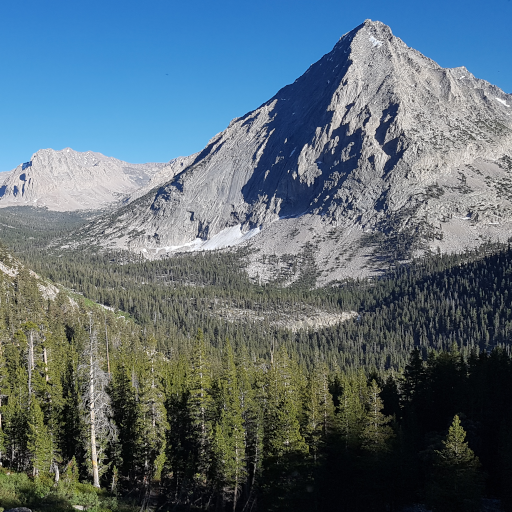
\includegraphics[width=\columnwidth]{graphics/johnmuirtrail.png}
        \caption{Input-Bild}
        \label{fig:input-bild}
    \end{subfigure}
    \begin{subfigure}{.5\columnwidth}
        \centering
        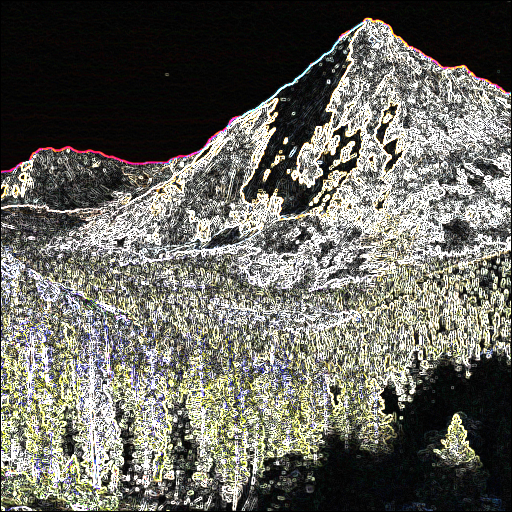
\includegraphics[width=\columnwidth]{graphics/johnmuirtrail_sobel.png}
        \caption{Output-Bild}
        \label{fig:output-bild}
    \end{subfigure}
\end{figure}

In Abbildung \ref{fig:input-bild} und \ref{fig:output-bild} ist ein Beispiel für die Anwendung des Sobel-Filters zu sehen.

\section{Lösungsansatz}
Unser gewählter Lösungsansatz besteht aus drei verschiedenen Versionen:
Die Basisversion (Version 0) implementiert den Sobel-Filter strikt nach seiner mathematischen Definition \ref{sec:math-def}.
Diese Version dient zusätzlich als Vergleichsimplementierung.
Die erste und zweite Version bauen jeweils aufeinander auf und zielen darauf ab, die Laufzeit der Basisversion bedeutend zu verbessern.
Version Eins verwendet Single Instruction Multiple Data (SIMD) Instruktionen, um eine größere Bandweite bei der Berechnung des Filters zu erreichen.
Dabei werden die Farbwerte von mehr als 5 Pixeln simultan berechnet und gespeichert.
Version Zwei kombiniert besagte erhöhte Bandbreite mit Multithreading, um die hohe Parallelität moderner Prozessoren optimal auszunutzen.

Jede der drei Versionen hat ein Gegenstück (Version 3 - Version 5), dass mit Graustufenbildern (8-Bit BMP) arbeitet.
Sie werden in der Performanzanalyse behandelt.
Diese Versionen sind nicht weiter für diesen Teil interessant, da sie exakt die selben Operationen durchführen und sich lediglich in der Anzahl der Bits pro Pixel unterscheiden.

\subsection{Vergleichsimplementierung}
\label{sec:vergleichsimplementierung}
Die Vergleichsimplementierung ist eine naive Implementierung des Sobel-Filter Algorithmus.
Diese ist bis auf einen kleinen Unterschied exakt nach der Definition \ref{sec:math-def} implementiert.
Um die Vergleichsimplementierung wirklich als Vergleich für die Optimierungen nutzen zu können verwendet die Vergleichsimplementierung eine Annäherung an den Pythagoras \ref{eq:wurzel}.
\begin{equation}
    O^{F}_{x,y} = \left | A^{v,F}_{x,y} \right | + \left | A^{h,F}_{x,y} \right |
    \label{eq:betrag}
\end{equation}
Grund dafür ist das Fehlen einer Instruktion zur Berechnung der Wurzel eines 16-Bit Wertes in der SSE2 Instruktionenmenge.
\begin{figure}[H]
    \begin{subfigure}{.5\columnwidth}
        \centering
        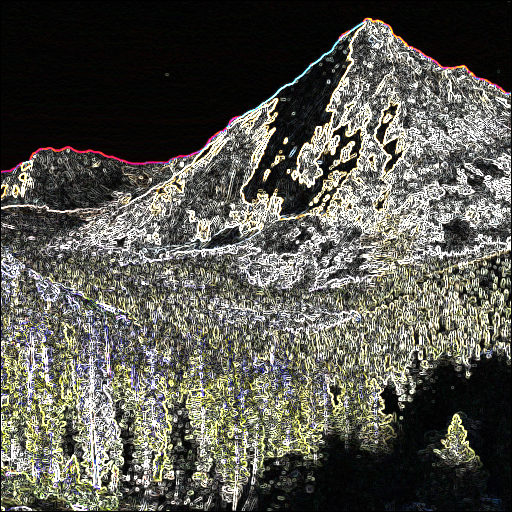
\includegraphics[width=\columnwidth]{graphics/sqrt_sobel.png}
        \caption{Pythagoras \ref{eq:wurzel}}
        \label{fig:sqrt-bild}
    \end{subfigure}
    \begin{subfigure}{.5\columnwidth}
        \centering
        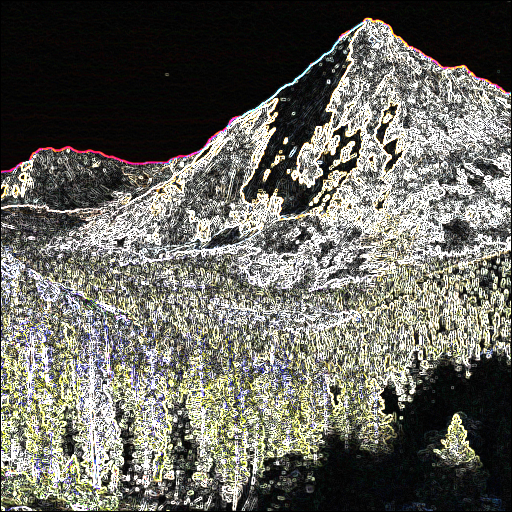
\includegraphics[width=\columnwidth]{graphics/johnmuirtrail_sobel.png}
        \caption{Annäherung \ref{eq:betrag}}
        \label{fig:abs-bild}
    \end{subfigure}
\end{figure}
Der Unterschied zwischen \ref{fig:abs-bild} und \ref{fig:sqrt-bild} liegt lediglich in der Helligkeit des Bildes, was für Kantenerkennung nicht relevant ist.
\subsection{SIMD Implementierung}
\label{sec:simd-implementierung}
Die SIMD Implementierung basiert auf der Vergleichsimplementierung, benutzt zur Berechnung jedoch SIMD Instruktionen.
Ein großes Problem bei der Arbeit mit 8-Bit-Ganzzahlen ist der kleine Wertebereich.
Da die Werte der einzelnen Farbchannel der Pixel als 8 Bit Integer gespeichert werden, kann es folglich bei der Faltungsoperation schnell zu einem Überlauf kommen.
Der naive Lösungsansatz, um dem entgegen zu wirken, ist das Input-Bild schlicht um 75\% zu verdunkeln. \label{sec:verdunkeln}
Durch die Verdunkelung wird der Überlauf zwar verhindert, das Output Bild ist jedoch auch (wesentlich) dunkler {\ref{fig:dark}}, wodurch die erkannten Kanten signifikant dunkler werden.
\begin{figure}[H]
    \begin{subfigure}{.5\columnwidth}
        \centering
        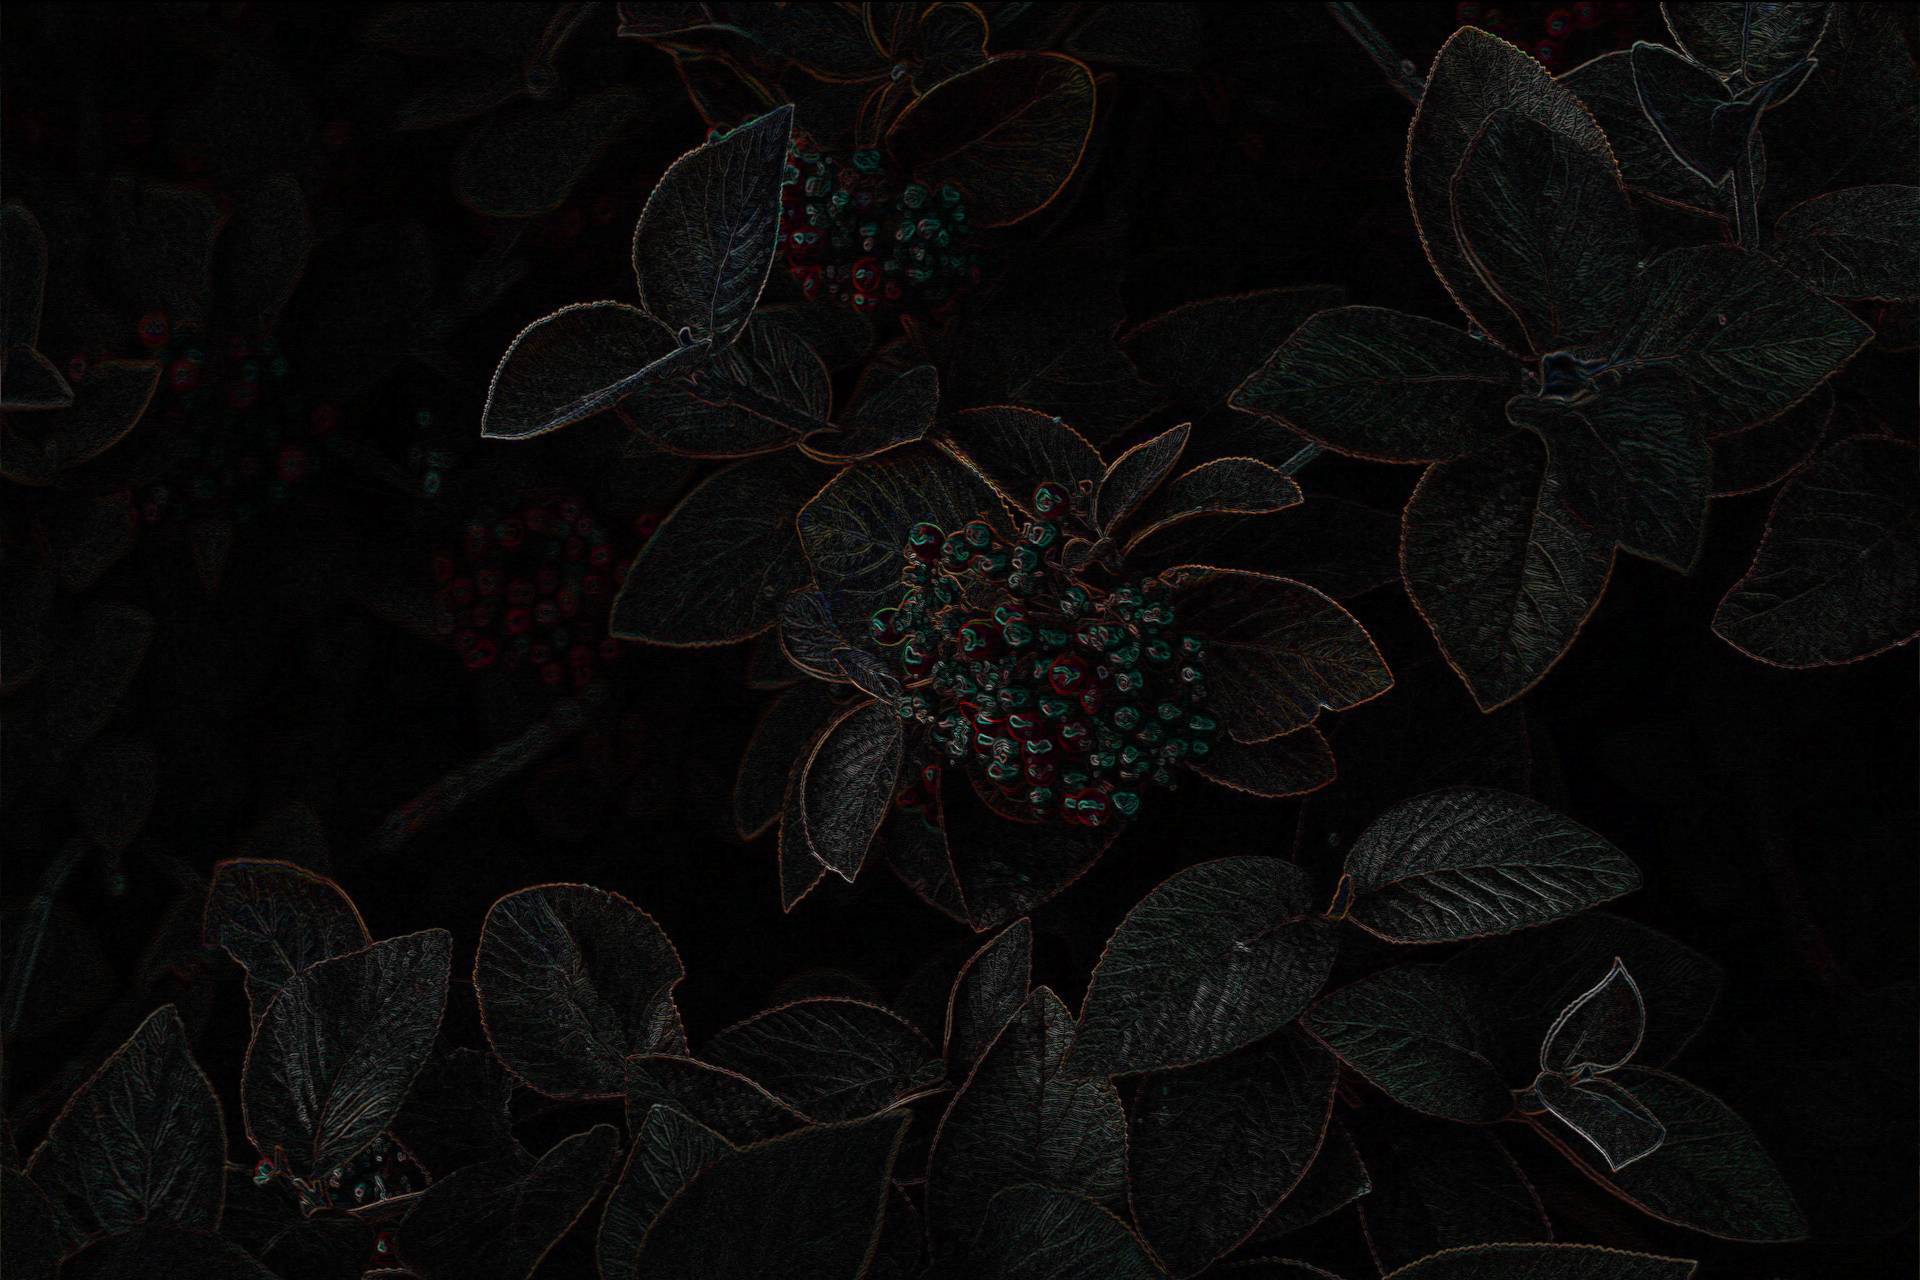
\includegraphics[width=\columnwidth]{graphics/dark.png}
        \caption{naiver SIMD Ansatz \ref{sec:verdunkeln}}
        \label{fig:dark}
    \end{subfigure}
    \begin{subfigure}{.5\columnwidth}
        \centering
        \includegraphics[width=\columnwidth]{graphics/correct.png}
        \caption{Vergleichsimplementierung \ref{sec:vergleichsimplementierung}}
        \label{fig:correct}
    \end{subfigure}
\end{figure}
Um trotz Vektorinstruktionen und sehr kleinen Wertebereichen ein Ergebnis zu erzielen,
das exakt der Vergleichsimplementierung entspricht, werden die Daten aus einem 16-Byte-Speicherbereich so in zwei Vektoren geladen, dass während der Berechnung je 8 Byte
als 16-Bit-Integer interpretiert werden können.
Dabei werden insgesamt 16 xmm Register benutzt, um jeweils die Sobel Werte für 16 Farbchannel gleichzeitig zu berechnen.
Das funktioniert so, dass ein 16 Byte-Speicherbereich gelesen wird und anschließend das jeweils höherwertige Byte eines jeden
16-Bit-Integers in diesem Vektor mit einer Bitmaske genullt wird.
Das geschieht analog mit den 16-Byte an der um einen Byte höheren Speicheradresse.
Für jeden der 16 Farbchannel, die mit einem Schleifendurchlauf berechnet werden können, werden so die acht umliegenden Farbchannel geladen.
Durch den entstehenden Overhead ist dieser Lösungsansatz zwar ca. nur halb so schnell, wie der naive SIMD-Ansatz, erzeugt jedoch ein korrektes Ergebnis, weshalb das Programm auch diesen Ansatz implementiert.

\subsection{SIMD-Implementierung mit Threading}
\label{sec:simd-threading}
Die SIMD-Implementierung mit Threading basiert auf der SIMD-Implementierung mit der Besonderheit, dass das Bild in Abschnitte eingeteilt werden, die jeweils von einem eigenen Thread bearbeitet werden.
Um diese Abschnitte zu erzeugen, wird das Bild in horizontale Streifen geschnitten.
Die Anzahl der Streifen wird von der Anzahl der durch die CPU bereitgestellten Threads bestimmt.
Dies führt zu einer Optimalen Auslastung der CPU.
Das horizontale Zerteilen des Bildes hat den Vorteil, dass der Cache besser genutzt wird, als zum Beispiel beim Aufteilen in Quadranten, weil die Daten hintereinander Zeile für Zeile im Speicher liegen.
Desweiteren besteht der Vorteil, fortlaufende Indizes bei der Berechnung nutzen zu können und nicht, wie zum Beispiel bei einer Aufteilung in Quadranten, diese Indizes aufwendig berechenen zu müssen.

\section{Genauigkeit}
Im folgenden wird die Genauigkeit unseres Lösungsansatzes analysiert, da es beim Sobel Operator keine fest definierte "source of truth", wie zum Beispiel bei einer Addition, gibt.
Die öffentlich existierende Sobel-Filter Implementierung von OpenCV liefert beispielsweise Ergebnisse, die sich leicht in der Helligkeit von unserer unterscheiden.
Desweiteren arbeitet diese auf Graustufenbildern, wohingegen unsere Implementierung auf RGB-Bildern arbeitet.
Wir haben die Implementierung von OpenCV so angepasst, dass sie ebenfalls auf RGB-Bildern arbeiten kann, um die Ergebnisse mit unseren zu vergleichen.
\begin{figure}[H]
    \begin{subfigure}{.5\columnwidth}
        \centering
        \includegraphics[width=\columnwidth]{graphics/basic.png}
        \caption{Vergleichsimplementierung}
        \label{fig:basic}
    \end{subfigure}
    \begin{subfigure}{.5\columnwidth}
        \centering
        \includegraphics[width=\columnwidth]{graphics/open_cv.png}
        \caption{Open CV Version}
        \label{fig:opencv}
    \end{subfigure}
\end{figure}
In \ref{fig:basic} ist die Vergleichsimplementierung zu sehen, in \ref{fig:opencv} die OpenCV Implementierung.
Es ist zu erkennen, dass die OpenCV Implementierung wesentlich dunkler (~50\%) ist als die Vergleichsimplementierung.
Da die Kanten dennoch korrekt (!und kontrastreicher!) erkannt werden und um unnötige Rechenschritte zu vermeiden, wird die Helligkeit der Vergleichsimplementierung nicht angepasst.
\\\\
Bei der Bewertung der Genauigkeit wird die Vergleichsimplementierung als Referenzpunkt verwendet.
Sie gilt als das korrekte Ergebnis und ist, um Fehler zu vermeiden, so simpel und leserlich gehalten wie nur irgendwie möglich.
Die mathematische Defintion, wie in \ref{sec:vergleichsimplementierung} beschrieben, wurde ohne weitere Optimierungen umgesetzt.
Des weiteren wurden Unittests hinzugefügt, die überprüfen, ob die Hilfsfunktionen korrekt implementiert sind.
Die optimierten Versionen SIMD \ref{sec:simd-implementierung} und SIMD mit Threading \ref{sec:simd-threading} erzielen Ergebnisse, die denen der Verlgiechimplementierung exakt entsprechen.
Um das zu erreichen, wird der in Version 1 implizit entstehende schwarze Rand explizit links und rechts nach der Berechnung hinzugefügt.
Da dafür - für Bilder mit herkömmlicher Größe - verschwindend wenig Schreiboperationen benötigt werden ist die Perfromanzeinbuße kaum messbar.
Es wird mit einem automatisierten Test überprüft, ob die Ergebnisse der SIMD und SIMD + Threading Versionen mit den
Ergebnissen der Vergleichsimplementierung übereinstimmen.
\section{Performanzanalyse}
Im folgenden Abschnitt wird die Performanz der einzelnen Lösungsansätze verglichen und analysiert.
Als gemeinsame Basis für alle Messergebnisse dient hierbei das mit GCC's Optimierungsstufe 3 kompilierte Programm, das auf einem AMD Ryzen 5 1600 mit 6 Kernen und 12 Threads ausgeführt wurde.
Bei den Messungen wurde großen Wert auf die Mindestlaufzeit von über einer Sekunde gelegt, um Messungenauigkeiten möglichst zu vermeiden.
Als Testdaten dienen Bilder mit verschiedenen gängigen Größenverhaltnissen (4:3, 16:9, 1:1, 3:4, 9:16, etc) und entsprechenden Auflösungen (1024x768, 1920x1080, 256x256, etc).
Diese Bilder werden mit zufälligen Pixeln gefüllt, was die Performanz jedoch nicht beeinflusst, da die Berechnung der Sobel-Werte unabhängig von den Pixelwerten ausgeführt wird.
Das ist insbesondere deshalb der Fall, weil der Algorithmus - sofern er auf unkomprimierten Bildern arbeitet - den Wert jedes Pixels einmal berechnen muss, wodurch auch die Laufzeit in O(n) liegen muss.
\begin{figure}[H]
    \centering
    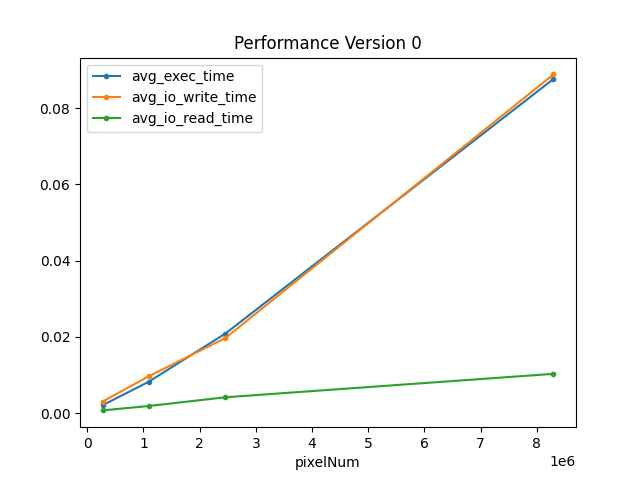
\includegraphics[width=0.5\columnwidth]{graphics/performance_vergleich}
    \caption{Performanz der Vergleichsimplementierung}
    \label{fig:performanz}
\end{figure}
Da die Vergleichsimplementierung schlicht die mathematische Definition des Verfahrens in C-Code übersetzt, wurden etwaige Verbesserungen wie Speicherzugriffsoptimierungen außenvor gelassen.
Die Daten des Bildes liegen Zeile für Zeile im Speicher, wobei die mathematische Definition über die einzelnen Spalten funktioniert.
Diese (kleine) Optimierung würde die Laufzeit der Vergleichsimplementierung um Faktor 2 beschleunigen, da dadurch Cachemisses signifikant reduziert werden können, aufgrund der Einfachheit wurde darauf jedoch verzichtet.
\begin{figure}[H]
    \centering
    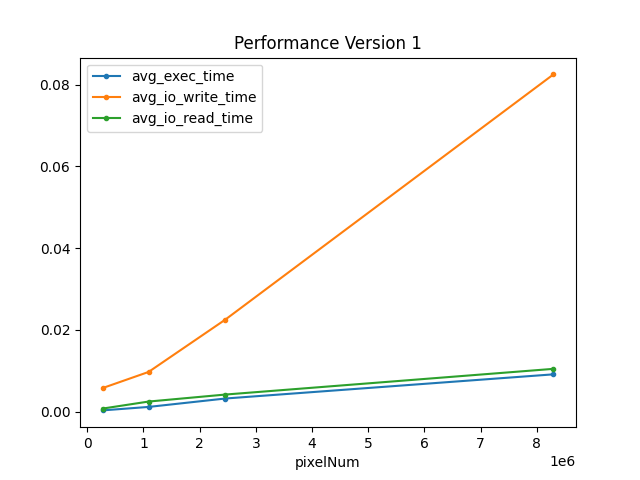
\includegraphics[width=0.5\columnwidth]{graphics/performance_simd}
    \caption{Performanz der SIMD-Implementierung}
    \label{fig:performanz-simd}
\end{figure}
Die SIMD-Implementierung erzielt in Relation zur Vergleichsimplementierung einen Speedup von circa 10.
Dies ist darauf zurückzuführen, dass zum einen die Berechnung der Sobel-Werte vektorisiert zum anderen aber auch die Speicherzugriffe optimiert werden (zeilenweiser statt spaltenweiser Zugriff).
Durch die Vektorisierung können 16 Farbchannel gleichzeitig verarbeitet werden, im Gegensatz zu der vollständig sequentiellen Berechnung der Vergleichsimplementierung.
Basierend auf dieser Information wäre der theoretisch maximale Speedup 16, was jedoch vom gemessenen Speedup von x10 abweicht, was auf den durch das versetzte Laden und aufbereiten der Vektoren entstehenden Overhead zurückzuführen ist.
Optimiert man die Speicherzugriffe der Vergleichsimplementierung, kann GCC ab Optimierungsstufe 3 interessanterweise die hohe Vektorisierbarkeit des Problems erkennen und übersetzt diese ebenfalls in Vektorinstruktionen.
Da der durch GCC generierte Ansatz jedoch nur 8 Byte gleichzeitig verarbeiten kann, ist unsere SIMD-Implementierung immer noch in etwa doppelt so schnell.

Die Threading-Implementierung kann durch ihren noch paralleleren Ansatz gegenüber der SIMD-Implementierung eine noch bessere Laufzeit mit einem Speedup von x2 (TO BE TESTED) erzielen.
Hierbei haben unsere Messungen ergeben, dass die optimale Anzahl an Streifen, in die das Bild aufgeteilt werden soll, den durch die CPU bereitgestellten Threads entspricht.
Dadurch kann die Parallelität von modernen CPUs bestmöglich ausgenutzt werden, während der Overhead für die Verwaltung der Threads möglichst gering bleibt.
Der durch diesen Ansatz theoretisch maximal mögliche Speedup gegenüber der SIMD-Implementierung entspräche der Anzahl an Threads, die die ausführende CPU bereitstellt.
Da jedoch nicht alle Threads dieselbe Rechenleistung liefern können, bzw. das Programm aufgrund des Schedulers nicht zu allen Zeitpunkten vollständig parallel arbeiten kann, weicht der gemessene Speedup stark vom theoretischen Maximum ab.
Des Weiteren ist es wichtig anzumerken, dass für besonders kleine Bilder die Threading-Implementierung - aufgrund des Thread-Verwaltungsoverheads - langsamer als die SIMD-Implementierung sein kann.

Bei der Rechereche zum Sobel-Operator fiel auf, dass so gut wie jede Implementierung Graustufenbilder zur Berechnung verwendet.
Deswegen wurden alle drei Versionen auch für Graustufenbilder implementiert.
(Bilder mit Performance)
Es zeigt sich, dass die Ausführungszeit auf den Graustufenbildern rund 1/3 der Ausführungszeit auf Farbbildern beträgt.
Somit wäre die Beschränkung auf Graustufenbilder ein einfacher Weg um eine signifikante Optimierung der Ausführungszeit zu erreichen.
Des Weiteren leidet die Kantenerkennung unter dem Fehlen der Farbe nicht, die Kanten sogar besser zu erkennen.

(2 Bilder mit Kante Farbe Kante grau)

Dies erklärt, warum so gut wie jede Impelementierung Graustufenbilder zur Berechnung benutzt.

Wie in der Einleitung bereits erwähnt, wird die Berechnung der Sobel-Werte normalerweise auf Graustufenbildern durchgeführt, da das die weitere Verarbeitung der erkannten Kanten erleichtert.
Durch diesen de-facto-Industriestandard produzieren die zusätzlichen Versionen (3-5) analog zu den Versionen 0-2 Graustufenbilder.
Da hierbei jedoch der einzige Unterschied die Pixelbreite - nämlich 8, statt 24 Bit - ist, entspricht der erwartete Speedup von 24/8 = 3 gegenüber der entsprechenden 24-Bit Implementierung genau dem gemessenen.
\section{Zusammenfassung und Ausblick}
TODO: Geben Sie hier eine kurze Zusammenfassung und einen Ausblick ein.
% TODO: Fuegen Sie Ihre Quellen der Datei Ausarbeitung.bib hinzu
% Referenzieren Sie diese dann mit \cite{}.
% Beispiel: CR7 ist ein portugiesischer Fußballspieler ~\cite{intel2017man}.
\bibliographystyle{plain}
\bibliography{Ausarbeitung}
\end{document}
